%%%%%%%%%%%%%%%%%%%%%%%%%%%%%%%%%%%%%%%%%
% FRI Data Science_report LaTeX Template
% Version 1.0 (28/1/2020)
% 
% Jure Demšar (jure.demsar@fri.uni-lj.si)
%
% Based on MicromouseSymp article template by:
% Mathias Legrand (legrand.mathias@gmail.com) 
% With extensive modifications by:
% Antonio Valente (antonio.luis.valente@gmail.com)
%
% License:
% CC BY-NC-SA 3.0 (http://creativecommons.org/licenses/by-nc-sa/3.0/)
%
%%%%%%%%%%%%%%%%%%%%%%%%%%%%%%%%%%%%%%%%%


%----------------------------------------------------------------------------------------
%	PACKAGES AND OTHER DOCUMENT CONFIGURATIONS
%----------------------------------------------------------------------------------------
\documentclass[fleqn,moreauthors,10pt]{ds_report}
\usepackage[english]{babel}
\usepackage{float}
\graphicspath{{fig/}}




%----------------------------------------------------------------------------------------
%	ARTICLE INFORMATION
%----------------------------------------------------------------------------------------

% Header
\JournalInfo{FRI Natural language processing course 2024}

% Interim or final report
\Archive{Project report} 
%\Archive{Final report} 

% Article title
\PaperTitle{LLM Prompt Strategies for Commonsense-Reasoning Tasks} 

% Authors (student competitors) and their info
\Authors{Jaša Samec, Haris Kupinić, and Jovana Videnović}

% Advisors
\affiliation{\textit{Advisor: Assist. Aleš Žagar}}

% Keywords
\Keywords{Keyword1, Keyword2, Keyword3 ...}
\newcommand{\keywordname}{Keywords}


%----------------------------------------------------------------------------------------
%	ABSTRACT
%----------------------------------------------------------------------------------------

\Abstract{

}

%----------------------------------------------------------------------------------------

\begin{document}

% Makes all text pages the same height
\flushbottom 

% Print the title and abstract box
\maketitle 

% Removes page numbering from the first page
\thispagestyle{empty} 

%----------------------------------------------------------------------------------------
%	ARTICLE CONTENTS
%----------------------------------------------------------------------------------------

\section*{Introduction}
	Due to their ability to generate human-like text and perform well on a variety of tasks, large language models, \textit{(LLMs)}, have become increasingly popular topics in recent periods.
	Nowadays, they are almost a daily tool for not just researchers, but millions of people.
	% TODO: Maybe add some Google Trends graphs.
	However, there are still some tasks that LLMs struggle with, such as simple math and logic, and commonsense reasoning.
	This is because LLMs are trained on large corpora of text and are not explicitly taught to reason about the world. 
	To improve their performance on these tasks, well-constructed prompts are effective.
	In this project, we explore different prompt strategies for improving the performance of LLMs on commonsense-reasoning tasks, including Chain of Thought (CoT) \cite{CoT}, in-context learning, and Plan-and-Solve (PS) \cite{plan-and-solve}.
	The effectiveness of these techniques is evaluated on commonsense reasoning datasets; including parts of CommonsenseQA \cite{commonsenseqa} and BIG-Bench \cite{bigbench} datasets.
	The model we employ is Llama 2 \cite{llama2}.

\begin{figure}[H]
  \centering
  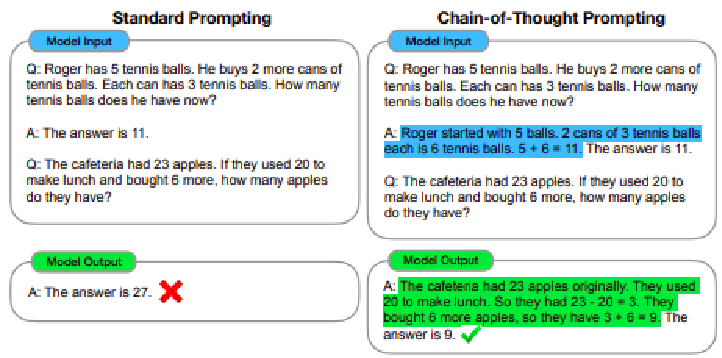
\includegraphics[width=1\linewidth]{fig/chain_of_thought.pdf} 
  \caption{Example of Chain of Thought approach. By splitting the problem into smaller subsets, model obtains the right result.}
  \label{fig:cot_example}
\end{figure}


%------------------------------------------------

\section*{Related work}
%\subsection*{Commonsense-reasoning in LLMs}
% Mogoce opisemo Big-bench ali CommonsenseQA?

\subsection*{Prompting methods}
To address the challenges that LLMs face in dealing with mathematical and logical reasoning tasks \cite{llm_bad_at_math}, researchers have suggested the use of prompts. Well-designed prompts have demonstrated to notably enhance the performance of LLMs, sometimes achieving results comparable to explicit fine-tuning \cite{few_shot_gpt3}. One fundamental prompting technique is \textit{in-context learning}, wherein the model is provided with example inputs and outputs before the desired output (e.g., supplying the model with example translations).

Another early technique in prompt engineering is Chain-of-Thought (CoT) prompting \cite{CoT}. This method adds a triple of the form \textit{(input, chain of thought, output)}, with the hope that when the model gets a new input (a question), it will follow it up with a chain of thought and then the output. The example CoT that is passed to the LLM breaks down the problem into smaller steps, making it easier to solve. This approach offers two benefits: first, the model can allocate more time/steps to the more difficult aspects of the problem. Second, it gives the user some insight into the model's reasoning process. 

Furthermore, from the Chain-of-Thought prompting, researchers began to develop zero-shot prompting strategies. The most known are zero-shot CoT \cite{kojima2023large} and Plan-and-Solve \cite{wang2023planandsolve}. Both of these methods guide the models response by asking it to think in smaller steps. Zero-shot CoT just starts the response by adding "Let's think step by step." While Plan-and-solve first guides the model to generate a list of possible steps and then asks it to follow them.

Later approaches such as Tree-of-Thought \cite{yao2023tree} and Graph-of-Thought \cite{besta2024graph} also break down the problem into smaller steps in different ways. For example, Tree-of-Thought asks the model to generate possible steps and then evaluates them. If a step is evaluated to be correct it builds upon it, otherwise the method backtracks through the previously chosen steps and generates new steps. Using this method the model generates a tree of logical steps that lead to the solution. 

However, newer methods such as Promptbreeder \cite{promptbreeder} have already surpassed the performance of some hand-crafted prompting techniques. This method combines the original prompt with different \textit{thinking styles} (e.g., "How could I measure progress on this problem?") and \textit{mutator prompts} (e.g., "How would you help an LLM to follow the instruction?") to generate new prompts by passing them to an LLM. Then, it scores the fitness of the generated prompts and iteratively mutates the best ones over multiple generations to evolve prompts specifically tailored to the task.

\section*{Methods}


%------------------------------------------------

\section*{Results}


%------------------------------------------------

\section*{Discussion}


%------------------------------------------------

\section*{Acknowledgments}


%----------------------------------------------------------------------------------------
%	REFERENCE LIST
%----------------------------------------------------------------------------------------
\bibliographystyle{unsrt}
\bibliography{report}


\end{document}